\section{Diagramm mit PIC-Code}
\pra
\subsection{Aufbau des PIC-Codes}
\noindent
Der Inhalt des generierten \textit{PIC}-Codes verfügt über eine gewisse Struktur. Zu Beginn des Dokuments werden erstmals alle \textit{Entities} und \textit{Beziehungstypen} definiert und gezeichnet. Diese sind noch mit keinem anderen Element verbunden. Sobald alle \textit{Entity}-Typen und \textit{Beziehungstypen} erstellt wurden, werden die Verbindungen zwischen den einzelnen Objekten gezeichnet. Der letzte Teil des Codes generiert die \textit{Attribute} und verbindet diese mit den jeweiligen \textit{Entity}-Typen. 
\\

\subsection{Problemfälle bei dem erstellten ERD}
\noindent
Das erzeugte \textit{Entity Relationship Diagramm} verfügt über gewisse Mängel. Diese entstehen zum Beispiel, indem sich gewisse Linien überschneiden. In diesem Fall besteht die Möglichkeit, dass der Inhalt der \verb|min|- und \verb|max|-Werte schwer lesbar wird. Abbildung \ref{Ueberschneidung} veranschaulicht dieses Problem.
\\


\begin{figure}[H]
	\begin{center}
		
\includegraphics{images/Ueberschneidung.png}
		\caption{min- und max-Werte schwer lesbar}
		\label{Ueberschneidung}
	\end{center}
\end{figure}
\pra
\noindent
Des weiteren kann es vorkommen, dass \textit{Attribute} sich überschneiden. Diese Überschneidungen können dazu führen, dass der Name eines \textit{Attributes} teilweise nicht mehr lesbar ist. Dieses Problem wird in Abbildung \ref{Attr_ueber} gezeigt.
\\

\begin{figure}[H]
	\begin{center}
		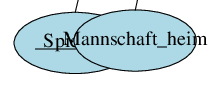
\includegraphics{images/Attr_ueber.png}
		\caption{Name der Attribute schlecht lesbar wegen Überschneidung}
		\label{Attr_ueber}
	\end{center}
\end{figure}

\noindent
\textit{Attribute} können am Rand der Grafik gezeichnet werden, sodass diese nur teilweise in dem angezeigtem Bereich liegen. Diesen Problemfall veranschaulich Abbildung \ref{Attr_abgeschnitten}.
\\

\begin{figure}[H]
	\begin{center}
		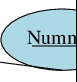
\includegraphics{images/Attr_abgeschnitten.png}
		\caption{Attribut liegt nur teilweise im sichtbaren Bereich}
		\label{Attr_abgeschnitten}
	\end{center}
\end{figure}


\subsection{Ist PIC-Code für das Projekt geeignet?}
\pra
\subsubsection{Generierung der Objekte des ERDs}
\textit{PIC} verfügt über viele einfache Mittel, um ein \textit{Entity Relationship Diagram} zu generieren. Auf Grund der bereits vordefinierten Objekte lässt sich das Zeichnen des Grundgerüstes des \textit{ERDs} relativ leicht gestalten. Bei der Implementierung einer Raute, die \textit{PIC} von Beginn an nicht bekannt ist, besteht ebenfalls kein großer Aufwand, wie in Abbildung \ref{Diamant_PIC} bereits erwähnt wurde.


\subsubsection{Zeichnen der Beziehungen}
\noindent
Weiters vereinfacht das Arbeiten mit Labels die Implementierung der Verbindungen zwischen den Elementen. Zuerst werden alle Boxen, Ellipsen und Rauten gezeichnet und sobald alle Elemente erstmals vorhanden sind, werden die Verbindungen zwischen den Objekten generiert. Auf Grund der Label ist dies kein Problem mehr, da auf die unterschiedlichen Elemente leicht zugegriffen werden kann (siehe Abbildung \ref{Label}).


\subsubsection{Skalierung der Objekte}
\noindent
Die Elemente können in \textit{PIC} leicht über das Argument \textit{scale} skaliert werden. Dies ist hilfreich, wenn die Größe des zu zeichnenden Diagrammes bereits bekannt ist. Jedoch kann nicht automatisiert skaliert werden. Das heißt, dass die Größe des \textit{ERDs} zuerst festgelegt werden muss. Da die Koordinaten im vorhinein schon erzeut werden, ist dies kein Problem, jedoch bringt diese Methode einen größeren Implementierungsaufwand mit sich.

\subsubsection{Zeichnen von Rauten/Dreiecken in Farbe}
\noindent
Im Gegensatz zu den Boxen und Ellipsen kann das farbige Zeichnen von Rauten und Dreiecken nicht umgesetzt werden, weil diese Elemente im Endeffekt nur Linien sind und auf die Position innerhalb der Linien nicht zugegriffen werden kann. Die unsichtbare Box, in der die Raute beziehungsweise das Dreieck gezeichnet werden, kann zwar farbig erstellt werden, jedoch wird dann nicht nur der Bereich innerhalb der Raute oder des Dreiecks gefärbt, sondern die ganze Box.

\subsubsection{Vergleich mit anderen Varianten}
\pra
\noindent
Im Vergleich zu den anderen Varianten \textit{Graphviz, Graphml} und \textit{Libre Office Draw} verfügt die Sprache \textit{PIC} über weniger Möglichkeiten für die Implementierung und Generierung eines \textit{Entity Relationship Diagrammes}. Beispielsweise kann das erzeugte Diagramm im Nachhinein nicht mehr verändert werden, da es in einer \textit{PDF}-Datei oder in ein Bild gespeichert wird. Bei den Varianten \textit{GraphML} und \textit{Libre Office Draw} können einzelne Elemente nachträglich noch per Hand verschoben werden. Daher ist \textit{PIC} im Vergleich zu den anderen Implementierungsvarianten am Wenigsten geeignet für dieses Projekt, jedoch gelingt es trotzdem, ein übersichtliches \textit{ERD} zu erzeugen.
\\

\subsubsection{Fertiges ERD}

\noindent
In Abbildung \ref{erd-pic} wird das mittels \textit{PIC}-Code generierte \textit{Entity Relationship Diagramm} von dem Datenmodell \textit{Fußball}  mit \textit{Attributen} und Farbe dargestellt.
\\

\begin{figure}[H]
	\begin{center}
		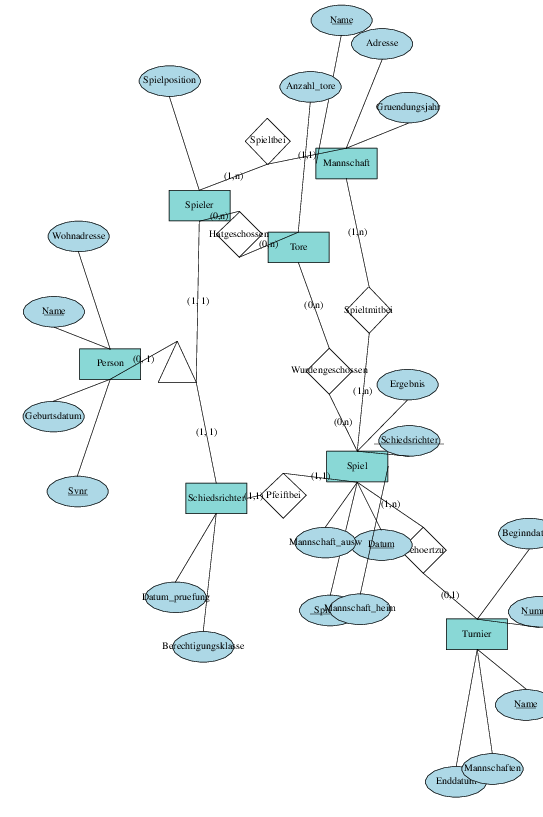
\includegraphics{images/fussball-erd.png}
		\caption{Mittels PIC erstelltes ERD für das Datenmodell Fußball}
		\label{erd-pic}
	\end{center}
\end{figure}
\pra
